\normaltrue
\correctiontrue

%\UPSTIidClasse{12} % 11 sup, 12 spé
%\newcommand{\UPSTIidClasse}{12}

\exer{Mouvement R  $\star$ \label{C1:05:02:PFD}}
\setcounter{numques}{0}
\UPSTIcompetence[2]{B2-14}
\UPSTIcompetence[2]{C1-05}
\index{Compétence B2-14}
\index{Compétence C1-05}
\index{Principe fondamental de la dynamique}
\index{PFD}
\index{Mécanisme à 1 rotation}
\ifcorrection
\else
\textbf{Pas de corrigé pour cet exercice.}
\fi

\ifprof
\else
Soit le mécanisme suivant. On a $\vect{AB}=R\vect{i_1}$ avec $R=\SI{20}{mm}$. La liaison pivot est motorisée par un moteur modélisée dont l'action mécanique sur \textbf{1} est donnée par $\vect{C_m}=C_m \vect{k_0}$.
On note $m_1$ la masse du solide \textbf{1} et $B$ son centre d'inertie. 
 La pesanteur est telle que $\vect{g}=-g\vect{j_0}$.
%On note $m_1$ la masse du solide 1, $B$ son centre d'inertie et $\inertie{G}{1}=\matinertie{A_1}{A_1}{A_1}{0}{0}{0}{\bas{1}}$.

\begin{center}
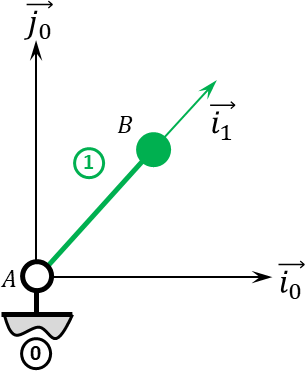
\includegraphics[width=\linewidth]{02_R_01}
\end{center}

\fi
\question{Réaliser le graphe d'analyse en faisant apparaître l'ensemble des actions mécaniques.}
\ifprof
\begin{center}
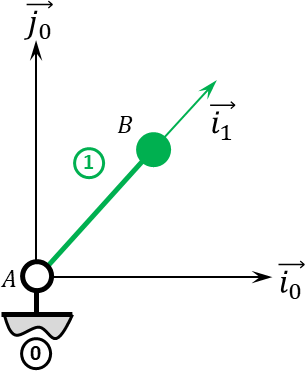
\includegraphics[width=6cm]{02_R_01}
\end{center}
\else
\fi

\question{Proposer une démarche permettant de déterminer la loi du mouvement de \textbf{1} par rapport à $\rep{0}$.}
\ifprof
On isole 1 et on réalise un théorème du moment dynamique en $A$ en projection sur $\vk{0}$.
\else
\fi


\ifprof
\else
\begin{flushright}
\footnotesize{Corrigé  voir \ref{C1:05:02:PFD}.}
\end{flushright}%
\fi